\section{Topologia: Computação como uma mercadoria}

O conceito da nuvem é construído sobre camadas, cada uma fornecendo um nível
distinto de funcionalidade. Essa estratificação dos componentes da nuvem forneceu o
meio para que as camadas da computação em nuvem se tornem uma mercadoria, como
eletricidade, serviço telefônico ou gás natural. A mercadoria que a computação em
nuvem vende é poder computacional a um custo e despesas menores para o usuário.
Espera-se que a computação em nuvem se torne o próximo serviço megautilitário.

Este é um exemplo da IBM: o virtual machine monitor (VMM). Ele fornece o meio para
uso simultâneo das instalações de nuvem (figura \ref{fig:vmm}). VMM é um programa em
um sistema host que permite que um computador suporte diversos ambientes de execução
idênticos. Do ponto de vista do usuário, o sistema é um computador autocontido que
é isolado dos outros usuários. Na realidade, cada usuário está sendo servido pela
mesma máquina. Uma máquina virtual é um sistema operacional (OS) que está sendo
gerenciado por um programa de controle subjacente, permitindo que ele pareça ser
diversos sistemas operacionais. Na computação em nuvem, o VMM permite que usuários
monitorem e gerenciem aspectos do processo, tais como acesso a dados, armazenamento
de dados, criptografia, endereçamento, topologia e movimento de carga de trabalho. 


\begin{figure}[ht]
    \centering
    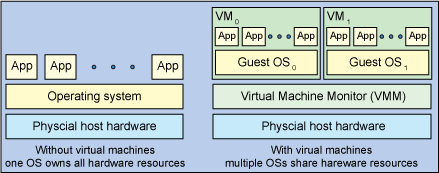
\includegraphics[width=0.6\textwidth]{img/vmm.png}
    \caption{Como o Virtual Machine Monitor funciona.}
    \label{fig:vmm}
\end{figure}


As camadas principais que a nuvem oferece são:

\newcommand{\itemm}[1]{\item\textbf{#1}}

\begin{itemise}
    \itemm{IaaS --- Infrastructure as a Service} (Infraestrutura como Serviço): A
    camada de infraestrutura é a base da nuvem. Ela consiste nos ativos físicos —--
    servidores, dispositivos de rede, discos de armazenamento, etc. Ao usar IaaS,
    o cliente não controla de fato a infraestrutura subjacente, mas controla os
    sistemas operacionais, armazenamento, aplicativos de implementação e, até certo
    ponto, controla componentes de rede selecionados. 
    
    Serviços de Print On Demand (POD) são um exemplo de organizações que podem se
    beneficiar da IaaS. O modelo de POD é baseado na venda de produtos customizados.
    PODs permitem que pessoas abram lojas e vendam designs de produtos. Os lojistas
    podem carregar o número de designs que quiserem à medida que os criam. Muitos
    carregam milhares. Com recursos de armazenamento em nuvem, um POD pode fornecer
    espaço de armazenamento ilimitado.
    
    \itemm{PaaS --- Plataform as a Service} (Plataforma como Serviço): A camada
    intermediária é a da plataforma. Ela fornece a infraestrutura de aplicativo.
    PaaS fornece acesso a sistemas operacionais e serviços associados, além de uma
    maneira de implementar aplicativos para a nuvem usando linguagens de programação
    e ferramentas suportadas pelo fornecedor. Não é necessário gerenciar ou
    controlar a infraestrutura subjacente, mas o cliente tem controle dos
    aplicativos implementados e, até certo ponto, de configurações de ambiente de
    \emph{hosting} de aplicativos. 
    
    PaaS tem provedores como Elastic Compute Cloud (EC2) da Amazon. A pequena 
empresa de software é um empreendimento ideal para PaaS. Com a plataforma elaborada,
produtos de classe mundial podem ser criados sem o gasto adicional da produção
interna.
    
    \itemm{SaaS --- Software as a Service} (Software como Serviço): A camada
    superior é a camada de aplicativo, a camada que a maioria visualiza como a
    nuvem. Aplicativos são executados aqui e são fornecidos on demand para os
    usuários. Software como Serviço (SaaS) tem provedores como Google Pack, que
    inclui aplicativos que podem ser acessados pela Internet, ferramentas tais como
    Calendar, Gmail, Google Talk, Docs e muito mais.
\end{itemise}

\begin{figure}[H]
    \centering
    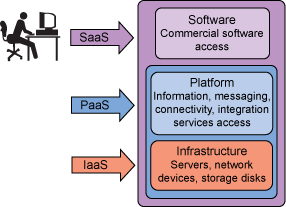
\includegraphics[width=0.7\textwidth]{img/layers.png}
    \caption{Principais camadas de computação em nuvem integradas nos componentes
        "como serviço"
    }
    \label{fig:layers}
\end{figure}


Existem também outros serviços oferecidos pela computação em nuvem:

\begin{itemise}

    \itemm{DevaaS - Development as a Service} (Desenvolvimento como Serviço): As
    ferramentas de desenvolvimento tomam forma na computação em nuvem como
    ferramentas compartilhadas, ferramentas de desenvolvimento web-based e serviços
    baseados em \emph{mashup}. 

    \itemm{CaaS - Communication as a Service} (Comunicação como Serviço): Uso de uma
    solução de Comunicação Unificada hospedada em Data Center do provedor ou
    fabricante (exemplo: Microsoft Lync). 

    \itemm{EaaS - Everything as a Service} (Tudo como Serviço): Quando se utiliza
    tudo, infraestrurura, plataformas, software, suporte, enfim, o que envolve
    T.I.C. (Tecnologia da Informação e Comunicação) como um Serviço. 

    \itemm{DBaas - Data Base as a Service} (Banco de Dados como Serviço): Quando
    utiliza a parte de servidores de banco de dados como serviço.

    \itemm{TaaS  - Testing as a Service}  (Ensaio como Serviço): Oferece um ambiente
    apropriado para que o usuário possa testar aplicações e sistemas de maneira
    remota, simulando o comportamento destes em nível de execução.

\end{itemise}


\begin{figure}[ht]
    \centering
    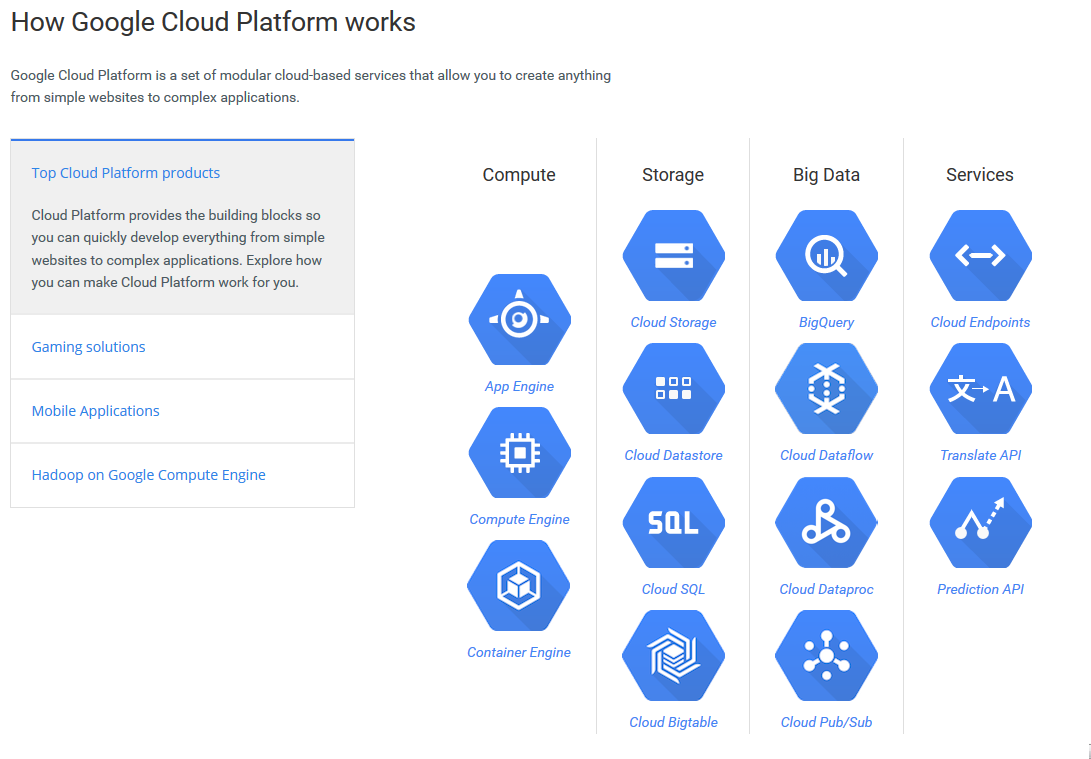
\includegraphics[width=0.8\textwidth]{img/googlecloud.png}
    \caption{Exemplo do provedor
             \href{https://cloud.google.com/}{Google~Cloud~Platform}
             para os serviços oferecidos para computação em nuvem
            }
    \label{img:googlecloud}
\end{figure}

\undef\itemm
